\section{Introduction}

\begin{frame}
\frametitle{Introduction}
\framesubtitle{What is a version control system (VCS)?}

\begin{block}{A software that allows to keep snapshots ("revisions") of a code base}
\begin{itemize}
\item Snapshots allow to split the development phase into small chunks with well-identified concerns
\item Previous snapshots can be consulted to help identify bugs, to restore previous code, etc.
\item Having well-identified milestones on the code base allows to compare and merge results from multiple developers
\end{itemize}
\end{block}

\end{frame}

\begin{frame}
\frametitle{Introduction}
\framesubtitle{No version control: typical scenarios of code development}

\begin{enumerate}
\item
\begin{block}{Overwriting the same source files over and over}
\begin{itemize}
\item You can't check why a certain bug has now surfaced in respect to a previous version
\item If another developer also works on a given file, identifying/importing/exporting changes can be difficult
\end{itemize}
\end{block}
\pause
\item
\begin{block}{Keeping numbered archives of the code base}
\begin{itemize}
\item Two developers must agree on a unique way of numbering, if they want to interact
\item You most likely need to archive the whole code base
\item Such archives inevitably end up thrown around your filesystem, possibly on multiple machines
\end{itemize}
\end{block}
\end{enumerate}

\end{frame}

\begin{frame}
\frametitle{Introduction}
\framesubtitle{What does a version control system offer?}

\begin{block}{Essentially:}
\begin{itemize}
\item To {\em commit} a snapshot, when desired, along with a comment 
\item To create {\em branches} of development where experimental features can be tested in isolation
\item To compare entire commits or specific files
\item To {\em merge} commits, either between different branches or between different developers
\end{itemize}
\end{block}

\end{frame}

\begin{frame}
\frametitle{Introduction}
\framesubtitle{Centralized versus distributed VCS}

\begin{block}{Centralized}
\begin{itemize}
\item Commits are directly sent to a central {\em repository} ({\em repo} for brevity) from where all developers get their code base
\end{itemize}
\end{block}

\begin{block}{Distributed}
\begin{itemize}
\item Each developer has its local copy of a {\em remote} repository, and commits remain local until {\em pushed} remotely
\end{itemize}
\end{block}

See also: \\  \url{http://en.wikipedia.org/wiki/Comparison_of_revision_control_software}.

\end{frame}

\begin{frame}
\frametitle{Introduction}
\framesubtitle{Advantages of a distributed VCS}

\begin{itemize}
\item You can work from any place, without the need of network connectivity until you need to "publish" your commits
\item A local copy of the repository means maximum speed of comparisons, checkout of branches, etc.
\item The distinction between a {\em commit} and a {\em push} encourages having frequent, small commits that allow to {\em amend} mistakes and facilitate merging
\end{itemize}

\end{frame}

\section{Git Tutorial}

\begin{frame}
\frametitle{Git}
\framesubtitle{Why Git?}

\begin{block}{Git is not the only DVCS out there}
\begin{itemize}
\item Open-source alternatives: notably Mercurial and Bazaar
\item Proprietary alternatives: notably BitKeeper
\end{itemize}
\end{block}
\pause
\begin{block}{Git has a growing spread}
\begin{itemize}
\item A lot of projects, both large and small, already use it
\item Many online code hosting services support it: e.g., Google Code, GitHub and BitBucket
\item It is integrated into several IDEs (natively or through a plugin)
\item It is well known in the online community, documented and supported
\end{itemize}
\end{block}
\end{frame}


\begin{frame}
\frametitle{Git}
\framesubtitle{Some setup and preferences}

\begin{block}{Set your username and email for identification (mandatory)}
\texttt{\$ git config ---global user.name "Name Surname"} \\
\texttt{\$ git config ---global user.email "surname.name@spes.uniud.it"}
\end{block}

\begin{block}{Add automatic full syntax coloring (helps a little)}
\texttt{\$ git config ---global color.ui true}
\end{block}
\pause
\texttt{---global} just means that these settings are valid for all repositories on your machine.
\end{frame}

\begin{frame}
\frametitle{Git}
\framesubtitle{Additional setup}

\begin{block}{For setting specific tools instead of the defaults (explained later)}
\texttt{\$ git config ---global core.editor vim} \\
\texttt{\$ git config ---global diff.tool vimdiff}  \\
\texttt{\$ git config ---global merge.tool vimdiff}
\end{block}

\pause
\begin{block}{Add some aliases for commands (optional)}
\texttt{\$ git config ---global alias.ci commit} \\
\texttt{\$ git config ---global alias.st status} \\
\texttt{\$ git config ---global alias.co checkout} \\
\texttt{\$ git config ---global alias.br branch} \\
\texttt{\$ git config ---global alias.cl clone} \\
\texttt{\$ git config ---global alias.log1 log ---oneline} \\
etc.
\end{block}
\end{frame}

\subsection{Creating repos}

\begin{frame}
\frametitle{Repository creation}

\texttt{\$ git init}

\bigskip
\begin{block}{It creates a new repository}
The repository is created in the current working directory, and will be responsible for all files and subdirectories within.
\end{block}
\begin{block}{The information is within the \texttt{.git} subdirectory}
In particular, the \texttt{.git/config} file contains configuration for the repository.
\end{block}
\end{frame}

\subsection{Status checking}

\begin{frame}
\frametitle{Status checking}

\texttt{\$ git status}

\bigskip
\begin{block}{It shows some relevant information}
\begin{itemize}
\item The current {\em branch} (more on that later)
\item New files not committed to the repository
\item Modified files
\item Removed files
\end{itemize}
At the moment we have the \texttt{Initial commit} text, and \texttt{nothing to commit} since no commit has been made and the repository is empty.
\end{block}

\end{frame}

\subsection{Staging}

\begin{frame}
\frametitle{Staging files}
\framesubtitle{What is staging?}

\begin{block}{Facts on version control systems}
\begin{itemize}
\item Files must be explicitly added to the repository (i.e., the file must be "tracked" or "added to the index"): being inside the directory of the repository does not make them part of it yet 
\item Such operation is called "tracking a file" or "adding a file to the index"
\item When a file is tracked, it can be chosen to be part of a commit (i.e., "staged")
\end{itemize}
\end{block}

\end{frame}

\begin{frame}
\frametitle{Staging files}
\framesubtitle{Adding files to the index}

\begin{block}{Create a new file and check the status}
\begin{tabular}{ll}
\texttt{\$ touch file1} & to create a new file \\
\texttt{\$ ls} & to see that it exists in the filesystem \\
\texttt{\$ git status} & to check what Git says about it
\end{tabular}

\medskip
Now you are informed that there are {\em untracked} files.
\end{block}

\pause

\begin{block}{Add it to the index and check the status}
\begin{tabular}{ll}
\texttt{\$ git add file1} & to track and simultaneously stage the file \\
\texttt{\$ git status} & to check what Git says about it
\end{tabular}

\medskip
Now you are informed that there are changes to be committed. The file now is both tracked (since it is new) and added to the stage area.
\end{block}

\end{frame}

\begin{frame}
\frametitle{Staging files}
\framesubtitle{Later modifications and removal from the staged area}

\begin{block}{What happens if we change a file that was added to the stage area}
\texttt{\$ echo "first line" >\;\!\!> file1} \\
\texttt{\$ git status} 

\medskip
Changing a staged file does not affect the {\em copy} of the file already in the stage area.
To incorporate the new changes, you must explicitly add the file again
\end{block}

\pause
\begin{block}{How to remove a file from the staged area}
\texttt{\$ git reset file1} \\
will restore the file as it was at the latest commit. Will not work until we have at least one commit!
\end{block}

\end{frame}

\subsection{Committing}

\begin{frame}
\frametitle{Committing files}
\framesubtitle{What is committing?}

\begin{block}{Some facts on version control systems}
\begin{itemize}
\item Committing practically stores a snapshot of the repository in the current state, with consideration to what has changed in the index
\item The information stored in a commit also includes a user-defined message summarizing the changes, the information on the {\em committer} (i.e., the developer), the commit time, the commit hash code (i.e., a unique version)
\item Committing allows at a later time to "re-roll" the repository to such state
\end{itemize}
\end{block}

\end{frame}

\begin{frame}
\frametitle{Committing files}
\framesubtitle{Performing the commit}

\begin{block}{Commit the changes in the index and check the status}
\texttt{\$ git commit -m "Significant message of your choice"} \\
\texttt{\$ git status}

\medskip
The commit itself shows some basic info on the operation, while the status now does not have either the \texttt{Initial commit} message or the info on the staged file.
\end{block}

\pause
\begin{block}{Messages should be meaningful}
Examples of what should be avoided:
\begin{itemize}
\item "Minor changes"
\item "Various fixes"
\item "Another commit"
\end{itemize}
otherwise identifying commits becomes difficult.
\end{block}

\end{frame}

\begin{frame}
\frametitle{Committing files}
\framesubtitle{Additional commits}

\begin{block}{Let's perform a couple of other commits}
\begin{enumerate}
\item \texttt{\$ git add file1} \\
\item \texttt{\$ git commit -m "Added a first line of text to file1"} \\
\item \texttt{\$ echo "Second line" >\;\!\!> file1} \\
\item \texttt{\$ echo "A" >\;\!\!> file2} \\ 
\item \texttt{\$ mkdir mydir} \\ 
\item \texttt{\$ git add file1 file2 mydir} \\
\item \texttt{\$ git commit -m "Modified file1 and created file2 and mydir"} 
\end{enumerate}
Note that you can add as many files as you want to the stage area. However, directories are not tracked (you need to add files within \texttt{mydir}).
\end{block}

\end{frame}

\begin{frame}
\frametitle{Committing files}
\framesubtitle{Checking the log}

\begin{block}{Git has plenty of ways to show the history of previous commits}
\begin{tabular}{ll}
\texttt{\$ git log} & the quickest \\
\texttt{\$ git log ---oneline} & the most compact \\
\texttt{\$ git log -n} & only the latest \texttt{n} commits \\
\texttt{\$ git log <file>} & the commits related to a file \\
\texttt{\$ git log ---graph} & the commit graph \\
\texttt{\$ git log ---decorate} & show branch and tag names \\
\texttt{\$ git show <commit>} & details on a commit
\end{tabular}

\medskip
and many more. Flags can be combined.
\end{block}
\end{frame}

\begin{frame}
\frametitle{Committing files}
\framesubtitle{Tags}

\begin{block}{Having commits identified by generated 40-bytes hexadecimal values is less than ideal}
Tags are references used to provide names to specific commits : \\
\texttt{\$ git tag <name> -m "Description"} \\

\medskip
\begin{itemize}
\item The name should be compact, like \texttt{working\_rtl}, or set as the release version, like \texttt{0.9.1-rc1}
\item The message is optional but useful to have some descriptive text when using \texttt{git show}
\item Tags are listed with \\
\texttt{\$ git tag}
\end{itemize}
\end{block}
\end{frame}

\begin{frame}
\frametitle{Committing files}
\framesubtitle{Amending a commit}

\begin{block}{What if the latest commit had some mistakes?}
For example, our latest message was incorrect. Then do: \\
\texttt{\$ git commit ---amend}

\medskip
It opens an editor (\texttt{nano} on Linux) to modify the message: we 
\begin{enumerate}
\item remove the "and mydir" part of the message,
\item save with Ctrl+X,
\item confirm with Y or y,
\item confirm the temporary file.
\end{enumerate}
Checking the log shows only the new commit. Precisely, the new commit is merged with the previous one. Your amendment can include modified files, new files, etc.: just add to the stage and amend.
\end{block}
\end{frame}

\subsection{Maintenance}

\begin{frame}
\frametitle{Miscellaneous maintenance}
\framesubtitle{Removing files}

\begin{block}{Removing files should be done in git}
Compare \\
\texttt{\$ rm file1} \\
\texttt{\$ git status} \\
with \\
\texttt{\$ git rm file2} \\
\texttt{\$ git status} 

\medskip
In the second case, the modification is already staged for commit. Otherwise, when many files are involved, adding missing files to the stage area becomes tedious.
\end{block}

\end{frame}

\begin{frame}
\frametitle{Miscellaneous maintenance}
\framesubtitle{Moving files}

\begin{block}{Files have history: you should keep it}
Instead of using: \\
\texttt{\$ mv file1 file10} \\
\texttt{\$ git rm file1 \&\& git add file10} \\
You should use: \\
\texttt{\$ git mv file1 file2}

\medskip
In the second case, the rename is already staged for commit. Also, if you commit and issue \\
\texttt{\$ git log ---follow file10} \\
you can see all the commits involving the current \texttt{file10}, even through renames.
\end{block}

\end{frame}

\begin{frame}
\frametitle{Miscellaneous maintenance}
\framesubtitle{Recovering from modifications}

\begin{block}{How to recover the removed files?}
\begin{itemize}
\item If modifications are not staged, like for \texttt{file2}, \\
\texttt{\$ git checkout --- file2}
\item Otherwise, we must unstage the modification first, with \\
\texttt{\$ git reset}
\end{itemize}
\end{block}

\pause
\begin{block}{Cleaning modifications and untracked files in batch}
\begin{itemize}
\item All modified tracked files can also be dropped with \\
\texttt{\$ git reset ---hard}
\item Untracked files can all be removed with \\
\texttt{\$ git clean -fd}
\end{itemize}
Attention: these commands are destructive!
\end{block}

\end{frame}

\begin{frame}
\frametitle{Miscellaneous maintenance}
\framesubtitle{Ignoring files}

\begin{block}{What if I have files around that I never want to stage?}
Typically, output binaries or other intermediate files.
\end{block}
\pause
\begin{block}{Create a \texttt{.gitignore} file on a directory}
\begin{itemize}
\item Within a \texttt{.gitignore} file you can insert a list of entries that identify file names that will be ignored by Git
\item You can use '\texttt{*}' for "any number of characters", '\texttt{?}' for "any one character", '\texttt{!}' in front of an entry to exclude a class of file names
\end{itemize}
\end{block}
\pause
\begin{block}{One \texttt{.gitignore} file per directory may be present}
The ignore rules are applied from the outermost \texttt{.gitignore} down to the innermost.
\end{block}

\end{frame}

\begin{frame}
\frametitle{Miscellaneous maintenance}
\framesubtitle{How ignoring works}

\begin{block}{Example:}
\begin{tabular}{ll}
\texttt{file0?} & any file starting with \texttt{file0} plus another char \\
\texttt{test.*} & any file starting with \texttt{test.}\\
\texttt{!test.tex} & except for \texttt{test.tex} \\
\end{tabular}
\end{block}

\pause
\begin{block}{Do not forget to track them}
\texttt{.gitignore} files should be kept within the repository
\end{block}
\pause
\begin{block}{Minor trick}
Create and track an empty \texttt{.gitignore} file in an empty directory in order to track an "empty" directory
\end{block}
\end{frame}

\subsection{Branching}

\begin{frame}
\frametitle{Branching}
\framesubtitle{What's branching for?}

\begin{block}{Branches allow for experimental development}
As with a tree, creating a new branch and committing to it does not change the branch we came from.
\end{block}

\begin{block}{How to create a branch, and show branches}
\begin{tabular}{ll}
\texttt{\$ git branch <mybranchname>} & to create \\
\texttt{\$ git branch} & to show all branches
\end{tabular}

\medskip
\begin{itemize}
\item The initial (and usually primary) branch is called {\em master}
\item Each branch holds a reference that points to the latest commit for the branch (the "tip")
\item A new branch points to the commit on which it was created
\item Each new commit on a branch moves the pointer accordingly
\end{itemize}
\end{block}

\end{frame}

\begin{frame}
\frametitle{Branching}
\framesubtitle{Check out a commit}

\begin{block}{To start working on a branch, we must move our state to it}
The repository state is a special reference called \texttt{HEAD}. A {\em checkout} moves \texttt{HEAD} to a specified commit:

\texttt{\$ git checkout <commit>}

\medskip
where the \texttt{<commit>} is a reference to a commit, i.e., a branch name or a tag or a hash value. A prefix of the hash can be used, if unique in the repo. 
\end{block}

\pause
\begin{block}{Checking out can be relative to a branch name}
\begin{tabular}{ll}
\texttt{\$ git branch other} & create a new branch \texttt{other} \\
\texttt{\$ git checkout master} & the latest commit on \texttt{master} \\
\texttt{\$ git checkout other} & the latest commit on \texttt{other} \\
\texttt{\$ git checkout master\textasciitilde{}} & the commit before the latest \\
\texttt{\$ git checkout master\textasciitilde{}2} & two commits before the latest
\end{tabular}
\end{block}
\end{frame}

\begin{frame}
\frametitle{Branching}
\framesubtitle{Use checkout to move around}

\begin{block}{In the end, we always check out a commit}
If such commit is the latest for the current branch, we can continue adding commits from there.
\begin{itemize}
\item Commits cannot (normally) be inserted in the middle of the commit tree: only on the leaves.
\end{itemize}
If it is not, we are in the {\em detached} state: \\
\texttt{\$ git checkout master\textasciitilde{}} \\
\texttt{\$ git branch}

\medskip
It is advisable to start making commits after having created a branch for them, otherwise it may become unreachable.
\end{block}

\end{frame}

\begin{frame}
\frametitle{Branching}
\framesubtitle{Continue development on a branch}

\begin{block}{We can start a branch from anywhere, not necessarily the latest of a branch}
\begin{enumerate}
\item \texttt{\$ git checkout master\textasciitilde{}} \\
\item \texttt{\$ git branch newbranch} \\
\item \texttt{\$ git checkout newbranch} \\
\item \texttt{\$ touch file3} \\
\item \texttt{\$ git add file3} \\
\item \texttt{\$ git commit -m "Added file3"} \\
\item \texttt{\$ git checkout master} \\
\item \texttt{\$ git log ---graph ---oneline ---decorate}
\end{enumerate}

The log command shows that the two branches have a different "history", namely \texttt{newbranch} starts from the second commit and then adds file3.
\end{block}
\end{frame}

\begin{frame}
\frametitle{Branching}
\framesubtitle{Continue development on the detached state}

\begin{block}{Commits cannot be inserted before the tip of a branch}
If we checkout something different from the plain name of the branch (i.e., to its tip), we are in the {\em detached} state: \\
\texttt{\$ git checkout master\textasciitilde{}} \\
\texttt{\$ git branch}
\end{block}
\pause
\begin{block}{You can still create commits in the detached state}
In the detached state, after having made some commits, we can re-attach the \texttt{HEAD} with: \\
\texttt{\$ git branch mynewbranch HEAD}
\end{block}

\end{frame}

\begin{frame}
\frametitle{Branching}
\framesubtitle{An example of a commit tree}

\begin{figure}
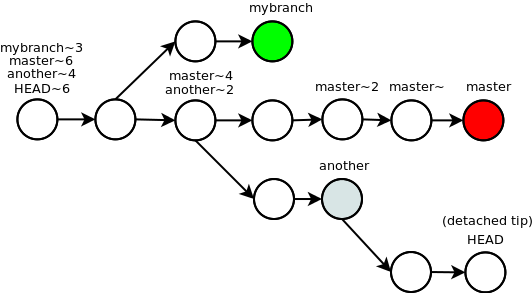
\includegraphics[width=0.7\textwidth]{lecture03/img/branches.png}
\end{figure}

\begin{itemize}
\item Since only one tree root exists, all back-references in the end reach it
\item Moving the \texttt{HEAD} out of the detached tip would make the commits unreachable on a later time
\end{itemize}

\end{frame}

\begin{frame}
\frametitle{Branching}
\framesubtitle{Merging}

\begin{block}{There may be a point when we want to {\em merge} results from a branch}
\texttt{\$ git checkout master} \\
\texttt{\$ git merge newbranch}  (if necessary, change the commit message)\\
\texttt{\$ git log ---graph ---oneline ---decorate}
\medskip

We always checkout the destination branch and indicate the source branch in the merge command. The log command shows that the two branches have merged, i.e., \texttt{master} incorporates the changes from \texttt{newbranch}.
\end{block}

\end{frame}

\begin{frame}
\frametitle{Branching}
\framesubtitle{An example of a graph after a merge}

\begin{figure}
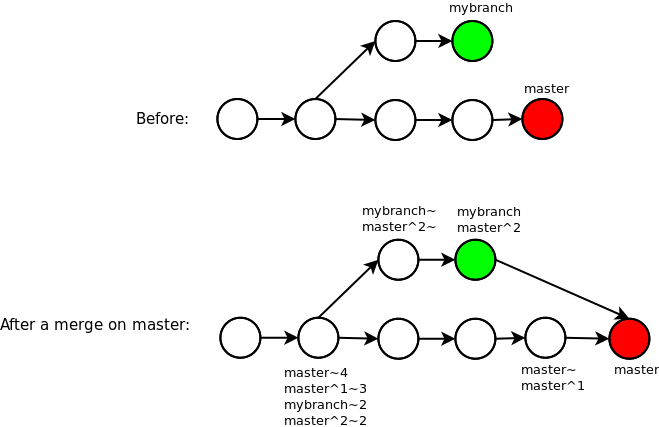
\includegraphics[width=0.7\textwidth]{lecture03/img/merging.png}
\end{figure}

\begin{itemize}
\item The \textasciicircum{}\texttt{n} symbol refers to the previous commit on parent branch number \texttt{n}
\item If no number is used, 1 is assumed, where 1 is always the referred branch: \texttt{master}\textasciicircum{}\texttt{1\textasciitilde{}2 = master}\textasciitilde{}\texttt{3}
\end{itemize}

\end{frame}

\begin{frame}
\frametitle{Branching}
\framesubtitle{Conflicts when merging}

\begin{block}{Not always changes from two branches are independent}
\begin{enumerate}
\item \texttt{\$ git checkout master}\\
\item \texttt{\$ echo "Third line" >\;\!\!> file1 \&\& git add file1} \\
\item \texttt{\$ git commit -m "Added third line to file1"}\\
\item \texttt{\$ git checkout newbranch}\\
\item \texttt{\$ echo "Another line" >\;\!\!> file1 \&\& git add file1} \\
\item \texttt{\$ git commit -m "Added another line to file1"}\\
\item \texttt{\$ git checkout master}\\
\item \texttt{\$ git merge newbranch}\\
\item \texttt{\$ git status}
\end{enumerate}

This causes a conflict because different text occupies the same position for the same file.
\end{block}

\end{frame}

\begin{frame}
\frametitle{Branching}
\framesubtitle{Resolving merge conflicts}

\begin{block}{Conflicts must be resolved by manual editing, followed by a commit}
\texttt{\$ nano file1} (and remove the parts that you don't want)\\
\texttt{\$ git commit -m "Merged changes from newbranch"}\\
\end{block}
\pause
\begin{block}{Alternatively use a merge tool (choose one from the list, recommended to install {\em meld})}
\texttt{\$ git mergetool}

\medskip
Here you can choose to copy the content from either of the conflicting files into the destination file. Then you commit as in the "manual" case.
\end{block}

\end{frame}

\begin{frame}
\frametitle{Branching}
\framesubtitle{Delete a branch}

\begin{block}{When development on a branch ends, you should clean up}
\texttt{\$ git branch -d newbranch} \\
\texttt{\$ git branch} \,\,\,(to see the absence of \texttt{newbranch})

\medskip
\begin{itemize}
\item Your \texttt{HEAD} must be on a branch different from the one to be deleted
\item You will be warned if commits from the branch have not been merged yet
\item If commits have been merged, only the reference of the branch is actually removed
\end{itemize}
\end{block}

\end{frame}

\subsection{Remote repos}

\begin{frame}
\frametitle{Remote repositories}
\framesubtitle{What is a remote repository?}

\begin{block}{A remote is a repository that different developers can use as common reference}
One developer works on a local copy (a {\em clone}) of the remote.
\end{block}
\begin{block}{Developers essentially use the remote as an intermediary}
They {\em push} their own changes to the remote, and {\em pull} from the remote the changes from other developers.
\end{block}

\end{frame}

\begin{frame}
\frametitle{Remote repositories}
\framesubtitle{How to create a remote repository}

\begin{block}{Empty repository}
\texttt{\$ mkdir myproject.git} \\
\texttt{\$ cd myproject.git} \\
\texttt{\$ git init ---bare}

\begin{itemize}
\item The \texttt{---bare} flag creates a repository with no working directory, equivalent to the \texttt{.git} hidden subdirectory
\item The \texttt{.git} extension of the directory is just a convention
\end{itemize}
\end{block}

\begin{block}{From an existing repository}
\texttt{\$ cd myotherproject} \\
\texttt{\$ git config ---bool core.bare true} \\
\texttt{\$ cp -R .git ../myotherproject.git}

\begin{itemize}
\item We set the repo as bare, then copy the \texttt{.git} directory
\end{itemize}
\end{block}

\end{frame}

\begin{frame}
\frametitle{Remote repositories}
\framesubtitle{How to clone a remote}

\begin{block}{Assuming to find a directory \texttt{myproject.git} (an empty bare repo) under the current directory}
\texttt{\$ git clone myproject.git} 

\begin{itemize}
\item Cloning can be done from remote locations too, using for example the HTTP/HTTPS or SSH protocols
\item The cloned directory is the same as the remote without the \texttt{.git} extension
\item An explicit directory name can be added as second argument of the \texttt{git clone} command
\end{itemize}
\end{block}

\begin{block}{Cloning is performed once for each copy of the remote we need}
We can create as many copies as we want, though.
\end{block}

\end{frame}

\begin{frame}
\frametitle{Remote repositories}
\framesubtitle{Pushing to a remote}

\begin{block}{Let's create a first commit and {\em push} it to the remote}
\texttt{\$ cd myproject} \\
\texttt{\$ touch file1 \&\& git add file1} \\
\texttt{\$ git commit -m "First commit"} \\
\texttt{\$ git push origin master}

\begin{itemize}
\item Here we "save" the current \texttt{master} branch to the remote, using its name \texttt{origin}
\item Successive pushes can be done by issuing \texttt{git push} only
\item Pushing with no arguments pushes all the commits that are missing in the remote
\end{itemize}
\end{block}

\pause
\begin{block}{Remote branches and their tips can be shown}
\texttt{\$ git branch -a} \,\,\, (\texttt{a} stands for {\em all} ) \\
\texttt{\$ git log ---graph ---oneline ---decorate}
\end{block}

\end{frame}

\begin{frame}
\frametitle{Remote repositories}
\framesubtitle{Pushing from another clone}

\begin{block}{Let's create another clone and push from it}
\begin{enumerate}
\item \texttt{\$ cd ..}
\item \texttt{\$ git clone myproject.git myproject2}
\item \texttt{\$ cd myproject2}
\item \texttt{\$ ls}
\item \texttt{\$ touch file2 \&\& git add file2}
\item \texttt{\$ git commit -m "Created file2"}
\item \texttt{\$ git push}
\end{enumerate}
\begin{itemize}
\item Here the clone includes the content of the remote as pushed by the first clone
\item We do not need to push the master branch, since it already exists on the remote
\end{itemize}
\end{block}

\end{frame}

\begin{frame}
\frametitle{Remote repositories}
\framesubtitle{Pulling from a remote}

\begin{block}{Pulling updates in respect to the remote}
\texttt{\$ cd ../myproject} \\
\texttt{\$ git pull} \\
\texttt{\$ git log ---oneline} \\
\texttt{\$ ls}

\begin{itemize}
\item Here we receive the content of the remote as pushed by the second clone
\end{itemize}
\end{block}

\end{frame}

\begin{frame}
\frametitle{Remote repositories}
\framesubtitle{Pulling includes merging}

\begin{block}{As with local merges, conflicts may arise}
\begin{enumerate}
\item \texttt{\$ echo "1" >\;\!\!> file3 \&\& git add file3} 
\item \texttt{\$ git commit -m "Created file3 on first clone"} 
\item \texttt{\$ git push} 
\item \texttt{\$ cd ../myproject2} 
\item \texttt{\$ echo "2" >\;\!\!> file3 \&\& git add file3}
\item \texttt{\$ git commit -m "Created file3 on second clone"}
\item \texttt{\$ git push}
\item \texttt{\$ git pull}
\end{enumerate}

\begin{itemize}
\item Pushing is not allowed if your local copy is behind
\item The merging in the pull operation fails due to \texttt{file3} having conflicting content
\end{itemize}
\end{block}

\end{frame}

\begin{frame}
\frametitle{Remote repositories}
\framesubtitle{Resolving the conflict}

\begin{block}{We therefore resolve and commit}
\texttt{\$ git mergetool} \,\,\,(and choose the preferred content)\\
\texttt{\$ git commit -m "Resolved conflict on file3"} \\
\texttt{\$ git log ---oneline} \\
\texttt{\$ git push \&\& cd ../myproject \&\& git pull} 

\begin{itemize}
\item Note that the order of commits now shows the \texttt{myproject} commit before the \texttt{myproject2} one
\item Pushing and pulling now have no issues, since \texttt{myproject2} is ahead of \texttt{myproject}
\end{itemize}
\end{block}

\end{frame}

\begin{frame}
\frametitle{Remote repositories}
\framesubtitle{Pushing new branches}

\begin{block}{New branches must be explicitly pushed}
\begin{enumerate}
\item \texttt{\$ git branch newbranch}
\item \texttt{\$ git branch -a}
\item \texttt{\$ git push -u origin newbranch}
\item \texttt{\$ cd ../myproject2}
\item \texttt{\$ git pull}
\item \texttt{\$ git branch -a}
\end{enumerate}

\begin{itemize}
\item The optional \texttt{-u} ("upstream") flag allows to configure \texttt{newbranch} to pull from \texttt{origin/newbranch} in the future
\item Note how the branch on the second clone has no local copy on \texttt{myproject2}: we can check it out with \\
\texttt{\$ git checkout origin/newbranch} \\
but it remains read-only since we are put in detached state.
\end{itemize}
\end{block}

\end{frame}

\begin{frame}
\frametitle{Remote repositories}
\framesubtitle{Tracking branches}

\begin{block}{New branches on \texttt{myproject2} must be manually tracked}
\texttt{\$ git branch ---track newbranch origin/newbranch} \\
\texttt{\$ git branch -a} \\
\begin{itemize}
\item \texttt{---track} sets up both push and pull, and is performed on a repo for which no local branch exists for the remote branch
\item The default of not tracking branches other than \texttt{master} is for cleanliness purposes: normally a branch is maintained by one developer only
\item The tracking operation must also be done for clones: the default is to clone \texttt{master} only
\end{itemize}
\end{block}

\end{frame}

\begin{frame}
\frametitle{Remote repositories}
\framesubtitle{Pushing/pulling tags}

\begin{block}{Tags can be pushed}
\texttt{\$ git push ---tags} \\

\medskip
while pulling them is done with a normal pull:

\begin{enumerate}
\item \texttt{\$ git tag v1.0 -m "First stable version"}
\item \texttt{\$ git tag}
\item \texttt{\$ git push ---tags}
\item \texttt{\$ cd ../myproject}
\item \texttt{\$ git pull}
\item \texttt{\$ git tag}
\end{enumerate}
\end{block}

\end{frame}

\subsection{Submodules}

\begin{frame}
\frametitle{Submodules}
\framesubtitle{What is a submodule?}

\begin{block}{A submodule is a nested repository}
It addresses the case of external dependencies that come from another repository
\end{block}
\pause

\begin{block}{Let's create a new remote repo with some commits}
\begin{enumerate}
\item \texttt{\$ cd ..}
\item \texttt{\$ mkdir mydependency.git \&\& cd mydependency.git}
\item \texttt{\$ git init ---bare}
\item \texttt{\$ cd ..}
\item \texttt{\$ git clone mydependency.git \&\& cd mydependency}
\item \texttt{\$ touch file1 \&\& git add file1}
\item \texttt{\$ git commit -m "Initial commit"}
\item \texttt{\$ git push origin master}
\end{enumerate}
\end{block}

\end{frame}

\begin{frame}
\frametitle{Submodules}
\framesubtitle{Add the submodule (on \texttt{master})}

\begin{block}{The directory of a submodule is treated differently}
\begin{enumerate}
\item \texttt{\$ cd ../myproject}
\item \texttt{\$ git checkout master}
\item \texttt{\$ git submodule add ../mydependency.git}
\item \texttt{\$ cd mydependency \&\& git status}
\item \texttt{\$ cd .. \&\& git status}
\end{enumerate}
\begin{itemize}
\item The \texttt{.gitmodules} file holds the configuration of modules within the repository
\item In practice, only the changes to the submodule directory are tracked
\end{itemize}
\end{block}
\end{frame}

\begin{frame}
\frametitle{Submodules}
\framesubtitle{Push and pull a submodule}

\begin{block}{There is a dedicated mechanism for pulling}
\begin{enumerate}
\item \texttt{\$ git commit -m "Added dependency submodule"}
\item \texttt{\$ git push}
\item \texttt{\$ cd ../myproject2}
\item \texttt{\$ git checkout master}
\item \texttt{\$ git pull}
\item \texttt{\$ git submodule init}
\item \texttt{\$ git submodule update}
\end{enumerate}
where the \texttt{init} operation is only needed if a new submodule is present in the \texttt{.gitmodules} file.
\begin{itemize}
\item The branches of the two clones must be the same, since \texttt{.gitmodules} is a regular versioned file
\end{itemize}
\end{block}
\end{frame}

\begin{frame}
\frametitle{Submodules}
\framesubtitle{Commit within the submodule}

\begin{block}{Submodules are initially set with a detached \texttt{HEAD}}
This way we must be explicit if we want to make changes to a dependency.

\medskip
\texttt{\$ cd ../myproject/mydependency} \\
\texttt{\$ touch file2 \&\& git add file2} \\
\texttt{\$ git commit -m "Added file2" \&\& git push} \\
\texttt{\$ cd .. \&\& git status} \\

\medskip
where we see that the \texttt{mydependency} directory is recognized as having new commits.
\begin{itemize}
\item Commits and pushes on the submodule are handled separated from those on the parent repository
\item Each commit on a dependency must be reflected by a commit on the parent repository: \\
\texttt{\$ git commit -am "Updated mydep" \&\& git push} \\
\end{itemize}
\end{block}

\end{frame}


\begin{frame}
\frametitle{Submodules}
\framesubtitle{Pulling changes from a repository with submodules}

\begin{block}{The updates require both a pull and an update}
\texttt{\$ cd ../myproject2} \\
\texttt{\$ git pull} \\
\texttt{\$ git submodule update}
\end{block}
\pause
\begin{block}{The above procedure is equivalent to the canonical:}
\texttt{\$ cd ../myproject2} \\
\texttt{\$ git pull} \\
\texttt{\$ cd mydependency} \\
\texttt{\$ git pull}

\medskip
but clearly is quicker if multiple dependencies are present.
\end{block}

\end{frame}

\subsection{Diffs and patches}

\begin{frame}
\frametitle{Diffs and patches}
\framesubtitle{What is a diff?}

\begin{block}{A diff identifies differences between any two commits}
For example, \\
\texttt{\$ git diff master\textasciitilde{} master} \\

\medskip
Essentially, text addition/removal is identified, along with the interested line. The order of the two commits counts: the difference is of the second commit in respect to the first. 
\end{block}

\pause
\begin{block}{Reading extensive diffs on multiple files is tedious}
You can exploit a diff tool with \\
\texttt{\$ git difftool master\textasciitilde{} master}

\medskip
which shows the diff for each file.
\end{block}

\end{frame}

\begin{frame}
\frametitle{Diffs and patches}
\framesubtitle{What is a patch}

\begin{block}{A patch incorporates one or more diffs, and can be applied by another party}
This is relevant if we want to submit changes to read-only repositories, as it normally happens for submodules.
\end{block}
\pause

\begin{block}{How to create a patch file}
The simplest way picks the \texttt{n} latest commits and creates a file \\
\texttt{\$ git format-patch -<n> ---stdout > myfile.patch} \\
\medskip
Opening the file shows that the \texttt{n} patches are present, one for commit, formatted as a sequence of email messages, for convenience purposes. 
Indeed, you could make git send patches via email.
\end{block}

\end{frame}

\begin{frame}
\frametitle{Diffs and patches}
\framesubtitle{How to apply a patch}

\begin{block}{Applying a patch is very simple}
On another clone where the patch file can be found at, e.g., \texttt{../mypatchfile.patch}, \\
\texttt{\$ git am ../myfile.patch} \\
which automatically creates corresponding commits for each patch in the file
\end{block}
\pause
\begin{block}{Commits in a patch are applied sequentially}
If one introduces conflicts, you must resolve them and issue \\
\texttt{\$ git am ---resolved} \\
or skip the patch with \\
\texttt{\$ git am ---skip} \\
While to restore the branch and stop patching: \\
\texttt{\$ git am ---abort}
\end{block}

\end{frame}

\begin{frame}
\frametitle{Diffs and patches}
\framesubtitle{An example}

\begin{block}{We purposefully create a conflict}
\begin{enumerate}
\item \texttt{\$ echo "Some text"  >\;\!\!> file4 \&\& git add file4} \\
\item \texttt{\$ git commit -m "Added file4 on myproject2"} \\
\item \texttt{\$ cp file4 file5 \&\& git add file5} \\
\item \texttt{\$ git commit -m "Added file5"} \\
\item \texttt{\$ git format-patch -2 ---stdout > file4and5.patch} \\
\item \texttt{\$ cd ../myproject} \\
\item \texttt{\$ echo "Some text"  >\;\!\!> file4 \&\& git add file4} \\
\item \texttt{\$ git commit -m "Added file4 on myproject"} \\
\item \texttt{\$ git am ../myproject2/file4and5.patch} \\
\item \texttt{\$ git am ---skip}
\end{enumerate}
\medskip
\pause
Here we skipped, but we could have removed \texttt{file4} from \texttt{myproject2}, for example.
\end{block}
\end{frame}
